

\documentclass[11pt]{beamer}

\usetheme{Madrid}
\usecolortheme{seahorse}
\setbeamertemplate{navigation symbols}{}

\usepackage[utf8]{inputenc}
\usepackage[T1]{fontenc}
\usepackage[ngerman,english]{babel}
\usepackage{amsmath,amssymb,bm,mathtools}
\usepackage{graphicx}
\usepackage{booktabs}
\usepackage{microtype}

\newcommand{\E}{\mathbb E}
\newcommand{\Var}{\operatorname{Var}}
\newcommand{\sigmoid}{\sigma}

\title[exact Bayesian
posterior sampling]{Exact Bayesian
posterior sampling
of Poissonian
random fields using
Polya Gamma data
augmentation}
\author[M. Holschneider, C. Chavez Chong, T. Luhdo, M. Opper]{Matthias Holschneider, Cristina Chavez Chong, Toni Luhdo, Mafred Opper}
\institute[UP]{University of Potsdam}
\date[]{October 15, 2026}

\AtBeginSection[]{
\begin{frame}{Outline}
\tableofcontents[currentsection]
\end{frame}
}

\begin{document}

\begin{frame}
\titlepage
\end{frame}

%\begin{frame}{Roadmap}
%\tableofcontents
%\end{frame}

% -------------------------------------------------
\section{Motivation}


\begin{frame}{Spatial Event Data}
Typical examples:
\begin{itemize}
\item Earthquakes occurences
\item Photon arrivals in imaging
\item Disease outbreaks
\item Crime hotspots
\end{itemize}

Observed data are often \textbf{point events}

Goal: infer an underlying smooth Poissonian intensity field.
$$
\Lambda(x) = 10^{a(x)}, \quad \mbox{or}\quad \Lambda(x, m) = 10^{a(x) - b(x) m}
$$
Assumption $\Lambda(x)$ and $\Lambda(x,m)$ are smooth functions.

\end{frame}

%\begin{frame}{Synthetic Point Catalog}
%\begin{center}
%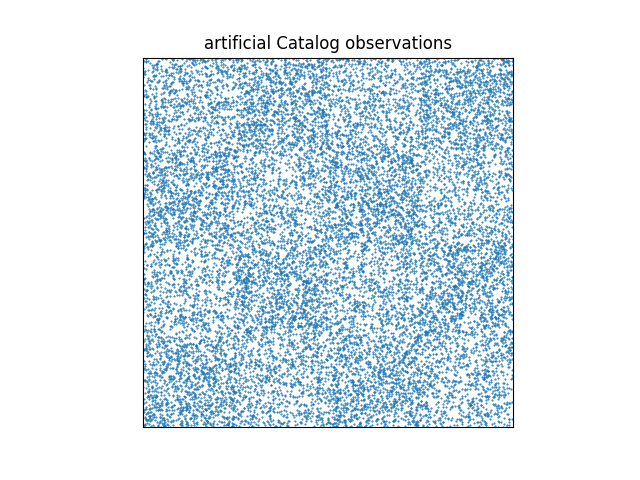
\includegraphics[width=0.72\textwidth]{figures/Figure_3.png}
%\end{center}

%We observe only events, not the rates.
%\end{frame}

% -------------------------------------------------
\section{Generative Model}


\begin{frame}{Latent Gaussian Field}
Latent Gaussian field $f(x)$ with prior Gaussian structur $\mathbb{P}(f)$
$$
\Lambda(x) =  L( f(x)), \quad f \sim \mathcal N(\mu(x),\Sigma(x,y))
$$
with some \textbf{non-linear} link function $L(f)$. Choices are
$$
e^{ f},\quad \lambda \sigma(f) = \frac{\lambda}{1+e^{-f}} \quad \log(1+e^{ f}) 
$$

Bayesian posterior ( $\sim$ Likelihood $\times$ Prior) of $f$ 
given a catalog of events $x_i$, $i=1,\dots, N$ is
$$
\mathbb{P}(f(x)| x_i) \sim \prod_i L(f(x_i)) e^{-\int L(f(x)) dx} \times \mathbb{P}(f(x))
$$

Goal: \textbf{efficient sampling} from this distribution.


\end{frame}

\begin{frame}{Discretization}

Finite dimensional approximation of field $f(x)$
$$
 f(x) =  \sum_k f_k \phi_k(x), \quad \phi_k(x) \quad \mbox{local basis functions}
$$
Choices of $\phi_k(x)$, finite elements (see previous talk of Sofiane), or our choice:
$$
\phi_k(x) = \mathbb{I}_{\Omega_k},\quad \mbox{piecewise constant appxoximation}
$$

\end{frame}

\begin{frame}{Discrete model for piecewise constant}

Counts in cells $\Omega_i$ are Poissonian
$$
n_i = \#\{ \mbox{events in $\Omega_i$} \} \sim \mbox{Poisson}(\gamma_i) = 
\frac{\gamma_i^{n_i} e^{-\gamma_i}}{n_i!}
$$
Poissonian rates $\gamma_i$ are obtained from discrete latent variables $f_i$
$$
\gamma_i = \lambda_i \sigma(f_i) = \frac{\lambda_i}{1+e^{-f_i}}
$$
Scaling of amplitude $\lambda_i$ with size of region $|Q_i|$
$$
\lambda_i \sim |Q_i|.
$$


Discrete proxy process multivariate Gaussian 
$$
f = [f_1, f_2, \dots f_M]^T  \sim \mathcal N( \mu, \Sigma_{ij})
$$

$\Sigma(x,y)$ $\Leftrightarrow$ discrete matrix $\Sigma_{i, j}$
valid for \textbf{correlation length $\gg$ size of pixel}
\[
\mu_i = \mu(x_i),\quad \Sigma_{i, j} \simeq \Sigma(x_i, x_j), \quad x_i\ \mbox{center of $Q_i$}
\]

\end{frame}

\begin{frame}{Efficient posterior sampling}

Posterior of $f_i$ given $n_i$ 
$$
\mathbb{P}(f_i | n_i) \sim \prod_i \lambda_i \sigma(f_i)^{n_i} e^{-\lambda_i \sigma(f_i)} 
e^{ -(f-\mu) \Sigma^{-1}(f-\mu) / 2}
$$

We propose \textbf{two stage data augmentation} scheme to \textbf{exactly} 
sample from this distribution without approximation (= no Laplace sheme etc).

The exponential part can be rewritten as (for fixed $f_i$ ) using
$$
\sigma(f_i) + \sigma(-f_i) = 1
$$
%and thus
%\begin{array}
%e^{-\lambda\sigmoid(f_i)} = e^{-\lmabda( 1 - \sigma(-f_i))}\\
%= e^{-\lambda}\,e^{\lambda\sigmoid(-f_i)} \\
%= C_{te}(f_i,\lambda)\sum_{k=0}^\infty \frac{(\lambda\sigmoid(-f_i))^k}{k!} e^{-\lambda\sigma(-f_i)}.
%\end{array}

and thus at fixed $f_i$
\[
\begin{array}{rl}
e^{-\lambda_i\sigma(f_i)} &= e^{-\lambda_i(1 - \sigma(-f_i))}\cr
&= e^{-\lambda_i}\,e^{\lambda_i\sigma(-f_i)} \cr
&= C_{te}(f_i,\lambda_i)\sum_{k=0}^\infty 
\frac{(\lambda_i\sigma(-f_i))^k}{k!} e^{-\lambda_i\sigma(-f_i)}.
\end{array}
\]
This suggests latent counts
\[
k_i\mid f_i \sim \operatorname{Poisson}(\lambda_i\sigmoid(-f_i)).
\]

\end{frame}

\begin{frame}
Together with the observed counts this gives the augmented likelihood
\[
\mathbb{P}(f_i \mid n_i, k_i)
\propto
\left(\sigmoid(f_i)\right)^{n_i}
\left(\sigmoid(-f_i)\right)^{k_i}
=
\frac{e^{n_i f_i}}{(1+e^{f_i})^{n_i+k_i}}.
\]

\medskip
This logistic form can be decomposed into Gaussians using the P\'olya--Gamma 
variables $PG(\omega| b, 0)$ ($b=n_i+k_i$). Gaussian mixture model
\[
\frac{e^{n f}}{(1+e^{f})^{n+k}}
= C_{te} e^{ (n-k) f / 2}
\int_0^\infty
\exp\left(
-\frac12\omega f^2 
\right)
PG(\omega\mid b,0)\,d\omega.
\]
We therefore have to sample from the tilted P\'olya--Gamma distribution
$$
\omega_i| k_i, f_i  \sim PG(\omega_i| b_i, f_i) \propto e^{-\omega_i f_i^2/2} PG(\omega_i\mid b_i,0).
$$
E.g. \textbf{polygamma.py or pypolyagamma.py} for Python package.
\end{frame}

\begin{frame}{The total scheme (exact!)}

For observed bincounts $n_i$ choose arbitrrary initial $f_i$ and then iterate through

$\bullet$ Sample \textbf{independent} auxiliary independent variables $k_i$
$$
k_i | f_i, n_i \sim \mbox{Poisson} ( \lambda_i \sigmoid(-f_i)).
$$
$\bullet$ Define $b_i=n_i+k_i$, $\kappa_i=(n_i-k_i)/2$.
Sample \textbf{independent} auxiliary random variables $\omega_i$ from the tilted Polyagamma distribution
\[
\omega_i\mid f_i,b_i,n_i \sim PG(b_i,f_i).
\]
$\bullet$ Sample the \textbf{collective/joint} $f_i$ from the modified Gaussian
\[
f\mid n,k,\omega \sim \mathcal N(m,Q^{-1}),
\qquad
m=Q^{-1}h.
\]
with (prior Gaussian $\mu$, $\Sigma$)
\[
Q=\Sigma^{-1}+\Omega,
\qquad
h=\Sigma^{-1}\mu+\kappa,
\qquad
\Omega=\operatorname{diag}(\omega_1,\dots,\omega_N).
\]

\end{frame}

\begin{frame}{Uniform ergodicity}

We can prove:

\begin{block}{Theorem (C. Chavez-Chong et al.)}
The sequence of samples $f^{(n)}$ are uniformly ergodic. 

Their distribution  converges 
exponentially fast to the invariant distribution of the chain.

This unique invariant distribution is the Bayesian posterior distribution.
\end{block}
\end{frame}


\begin{frame}{Choice of prior covariance I}

You may impose any prior covariance structure (either $\Sigma$ or $\Sigma^{-1}$)

Typical spatial kernels are ($r=|x_i-x_j|$)
\[
s^2\exp\!\left(-\frac{r^2}{2\rho^2}\right),
\qquad \frac{s^2 2^{1-\nu}}{\Gamma(\nu)} 
\left( \frac{\sqrt{2\nu}\, r}{\rho} \right)^{\nu}
K_\nu\!\left( \frac{\sqrt{2\nu}\, r}{\rho} \right)
\]
where

\begin{itemize}
\item $s^2$ = marginal prior variance
\item $\rho$ = correlation length
\end{itemize}

\end{frame}

\begin{frame}{Sparsity}

Only computational load is
\[
Q=\Sigma^{-1}+\Omega,
\qquad
h=\Sigma^{-1}\mu+\kappa,
\qquad
\Omega=\operatorname{diag}(\omega_1,\dots,\omega_N).
\]
And for sampling from the associated Gaussian $\mathcal{N}(h, Q^{-1})$
\[
Q = L L^T\quad \mbox{Cholesky decomposition}
\]


Therefore \textbf{sparsenesss} of precision matrix $\Sigma^{-1}$ is what pays off.

\begin{columns}[T]
\begin{column}{0.45\textwidth}
\begin{center}
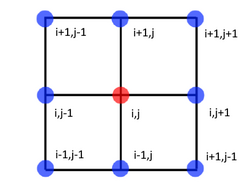
\includegraphics[width=\textwidth]{figures/9-point_stencil.png}
\end{center}
\end{column}
\begin{column}{0.55\textwidth}
\small

For Matern kernel
$$
\Sigma^{-1} = \gamma (\mathbb{I} - \alpha \Delta)
$$
$\Delta$ discrete Laplacian (e.g $9$ point stencil).

Correlation length in pixel $\rho\leftrightarrow\alpha$
$$
\alpha = (\cosh(1/\rho) -1)/2
$$

\end{column}
\end{columns}



\end{frame}

\end{document}

\begin{frame}{Choice of prior covariance III}

Chosing $\Sigma_{i,j}$ from continuous prior $\Sigma(x, y)$. Tentative approach through grid sampling 
$$
    \Sigma_{i,j} = \Sigma(x_i, y_i) 
$$
Valid approximation if and only if 
$$
\mbox{prior correlation lenght} \gg \mbox{grid size}
$$



$\Lambda(x) = L(f)$: offgrid random field $f$ with covariance $\mu, \Sigma(x,y)$
$$
\int_\Omega \Lambda(x) dx = \int_\Omega L(f(x) dx \not= L(\int_\Omega f(x) dx)
$$
Suppose stationary prior (i.e. kernel K=K(x-y)). Then
$$
\int_\Omega \Lambda(x) dx \sim \sqrt{|Q|},\quad \mbox{but} L(\int_\Omega f(x) dx) \sim L(\gamma \sqrt{\Omega})
$$

 

\end{frame}

\begin{frame}{Induced Local Priors on Intensity}
\begin{center}
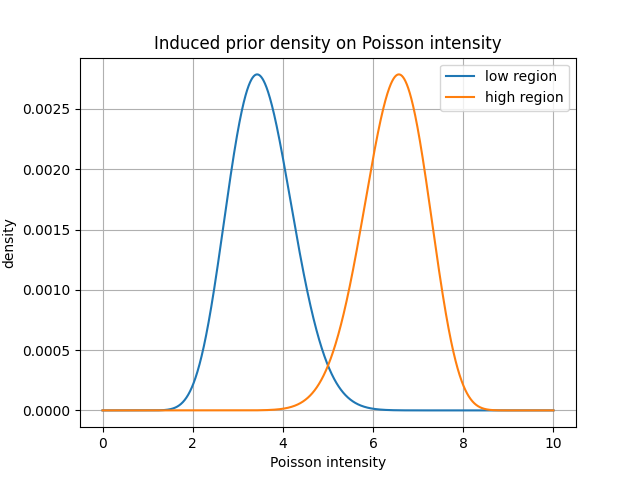
\includegraphics[width=0.42\textwidth]{figures/Figure_1.png}
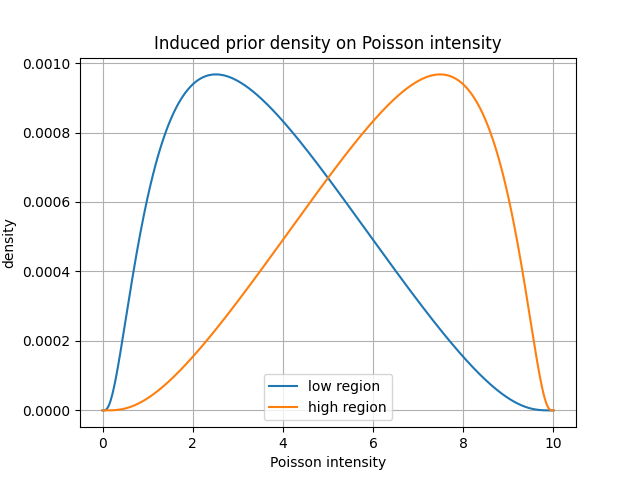
\includegraphics[width=0.42\textwidth]{figures/Figure_15.png}
\end{center}

The prior is Gaussian in the latent variable $f_i$, but the link function transforms it to the intensity scale:
\[
\lambda_i = \lambda\,\sigmoid(f_i).
\]

The two curves correspond to two different local prior means in latent space,
with the same one-dimensional variance:
% \[
% f_i \sim \mathcal N(\mu_{\mathrm{low}},v^2),
% \qquad
% f_i \sim \mathcal N(\mu_{\mathrm{high}},v^2).
% \]
\[
f_i \sim \mathcal N(\mu,v^2),
\]
\end{frame}

\begin{frame}{Synthetic Example: Structured Rate Field}
\begin{center}
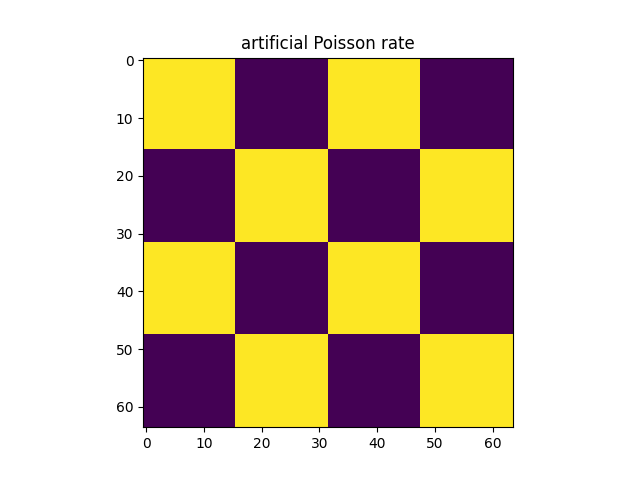
\includegraphics[width=0.61\textwidth]{figures/Figure_2.png}
\end{center}

We use the same checkerboard structure with two different contrast settings:
\[
\begin{array}{c|ccc}
& \lambda_{\mathrm{low}} & \lambda_{\mathrm{high}} & \lambda \\
\hline
\text{Example I} & 4.5 & 5.5 & 10 \\
\text{Example II} & 3.5 & 6.5 & 10
\end{array}
\]
\end{frame}


\begin{frame}{Discretization: From Point Events to Counts}
After discretization into grid cells:
\[
n_i = \#\{\text{events in cell } i\},
\qquad
n_i \sim \operatorname{Poisson}(\lambda_i)
\]
\vspace*{-15mm}
\begin{columns}[T]
    \begin{column}{0.49\textwidth}
    \begin{center}
    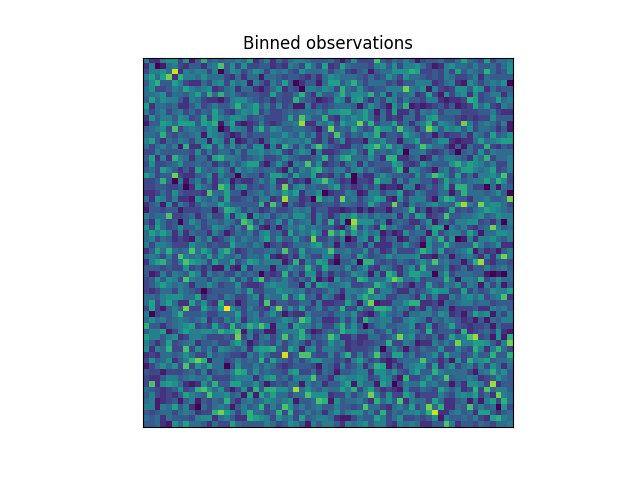
\includegraphics[width=\textwidth]{figures/Figure_11.png}
    \end{center}
    \end{column}
    \begin{column}{0.49\textwidth}
    \begin{center}
    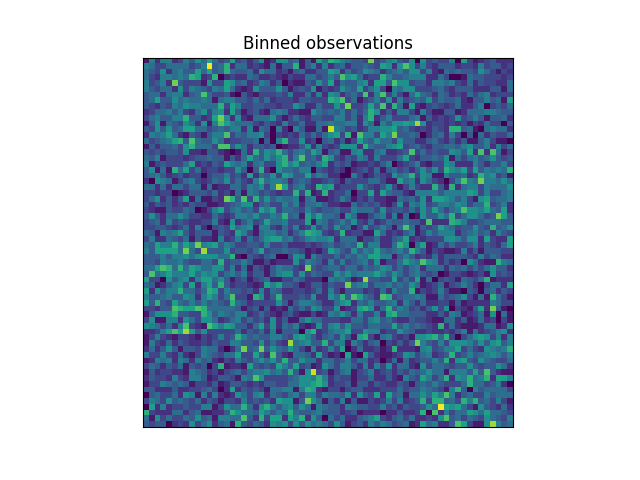
\includegraphics[width=\textwidth]{figures/Figure_4.png}
    \end{center}
    \end{column}
\end{columns}
\vspace*{-1mm}
The observations are discrete and noisy; the latent rate field is not observed.\\
\vspace*{2mm}
The generative model is now clear, but inference is not straightforward:\\
the Poisson--sigmoid likelihood is not conjugate to the Gaussian prior.
\end{frame}


% -------------------------------------------------
\section{Bayesian Inference}

\begin{frame}{Posterior Target}
We observe counts on grid cells and model
\[
n_i \mid f_i \sim \operatorname{Poisson}(\lambda\sigmoid(f_i)),
\qquad
f \sim \mathcal N(\mu,\Sigma).
\]

The posterior target is
\[
p(f\mid n) \propto p(n\mid f)\,p(f).
\]

The likelihood is, up to constants independent of $f$,
\[
\ell(f)=
\prod
 \sigmoid(f_i)^{n_i} e^{- \lambda\sigmoid(f_i)}.
\]

\medskip
\textbf{Obstacle:} the Poisson--sigmoid likelihood is not conjugate to the Gaussian prior.
\end{frame}

\begin{frame}{Poisson Splitting: From Poisson to Logistic Form}
The exponential part can be rewritten as (for fixed $f_i$ )
\[
e^{-\lambda\sigmoid(f_i)}
=
e^{-\lambda}\,e^{\lambda\sigmoid(-f_i)} = 
C_{te}(f_i,\lambda)\sum_{k=0}^\infty \frac{(\lambda\sigmoid(-f_i))^k}{k!} e^{-\lambda\sigma(-f_i)}.
\]

This suggests latent counts
\[
k_i\mid f_i \sim \operatorname{Poisson}(\lambda\sigmoid(-f_i)).
\]

Together with the observed counts this gives the augmented likelihood
\[
p(n_i\mid k_i, f_i)
\propto
\left(\sigmoid(f_i)\right)^{n_i}
\left(\sigmoid(-f_i)\right)^{k_i}
=
\frac{e^{n_i f_i}}{(1+e^{f_i})^{n_i+k_i}}.
\]

\medskip
This logistic form can be decomposed into Gaussians using the P\'olya--Gamma 
variables.
\end{frame}

\begin{frame}{P\'olya--Gamma Augmentation}
Define
\[
b_i=n_i+k_i,
\qquad
\kappa_i=\frac{n_i-k_i}{2}.
\]

The augmented likelihood has the standard P\'olya--Gamma form
\[
\frac{e^{n_i f_i}}{(1+e^{f_i})^{b_i}}
\propto
\int_0^\infty
\exp\left(
-\frac12\omega_i f_i^2 + \kappa_i f_i
\right)
p(\omega_i\mid b_i,0)\,d\omega_i.
\]

Equivalently, in the Gibbs sampler we draw
\[
\omega_i\mid f_i,b_i \sim PG(b_i,f_i).
\]

\medskip
\textbf{Key point:} conditional on $\omega$, the likelihood is quadratic in $f$.
\end{frame}

\begin{frame}{Gaussian Update and Cholesky Sampling}
Combining the quadratic likelihood with the Gaussian prior gives
\[
\log p(f\mid n,k,\omega)
=
-\frac12 f^\top Qf+f^\top h+c,
\]
with
\[
Q=\Sigma^{-1}+\Omega,
\qquad
h=\Sigma^{-1}\mu+\kappa,
\qquad
\Omega=\operatorname{diag}(\omega_1,\dots,\omega_N).
\]

Thus
\[
f\mid n,k,\omega \sim \mathcal N(m,Q^{-1}),
\qquad
m=Q^{-1}h.
\]

In practice we do not compute $Q^{-1}$ explicitly. We use
\[
Q=LL^\top
\]
and solve triangular systems.
\end{frame}

% -------------------------------------------------
\section{Results}

\begin{frame}{Gaussian First Guess}
\begin{columns}[T]
\begin{column}{0.45\textwidth}
\begin{center}
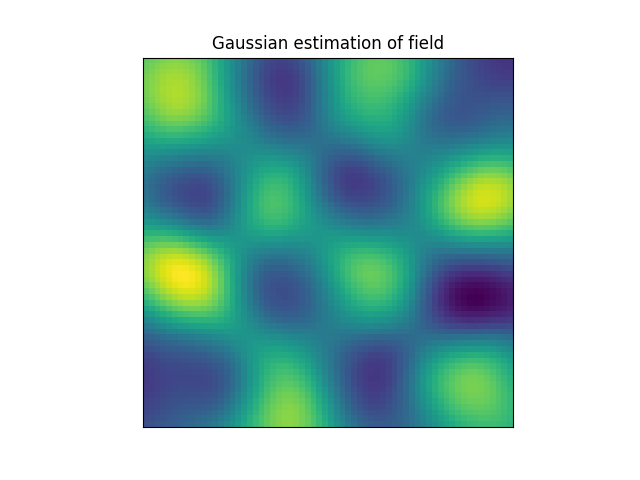
\includegraphics[width=\textwidth]{figures/Figure_5.png}
\end{center}
\end{column}
\begin{column}{0.55\textwidth}
\small
\begin{itemize}
\item Construct a pixelwise rate proxy from the observed counts:
\[
\lambda_i=\operatorname{clip}(n_i+1).
\]
\item Map it back to the latent scale:
\[
 f_i=\sigmoid^{-1}\!\left(\frac{\lambda_i}{\lambda}\right).
\]
\end{itemize}
\end{column}
\end{columns}
\begin{itemize}
\item Approximate local uncertainty by error propagation:
\[
s_i^2\approx\frac{\lambda_i}{\left(\frac{d\lambda_i}{df_i}\right)^2}.
\]
\item Combine this noisy proxy with the Gaussian prior to obtain a smoothed initialization.
\end{itemize}
\end{frame}

\begin{frame}{Posterior Samples}
\begin{center}
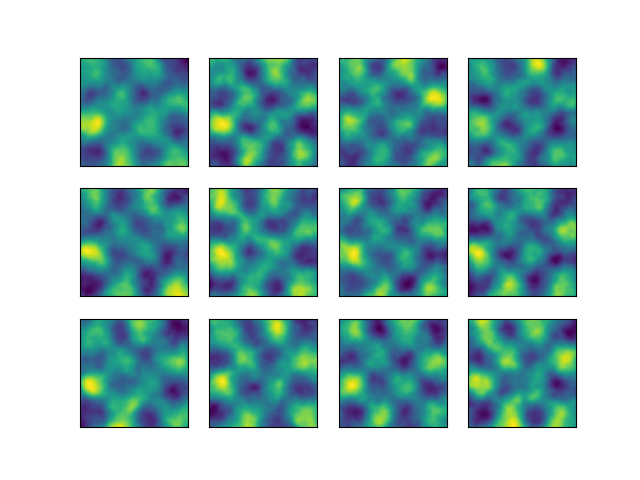
\includegraphics[width=0.82\textwidth]{figures/Figure_6.png}
\end{center}
\end{frame}

\begin{frame}{Posterior Mean Reconstruction: Example I}
Recovered spatial structure from event data.
The posterior mean is smoother than the discrete observations and reflects the spatial prior.

\begin{center}
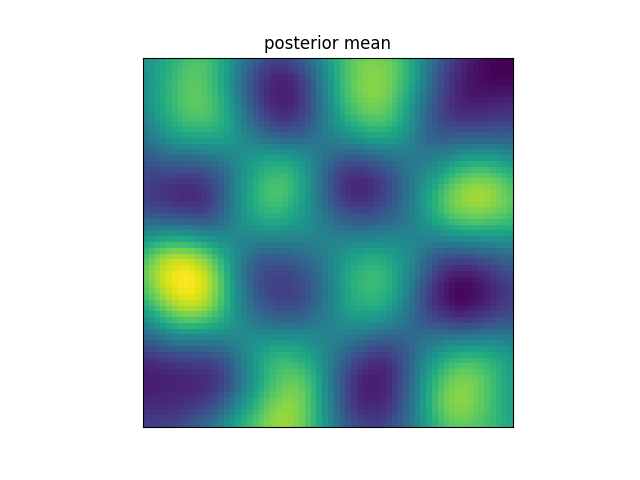
\includegraphics[width=0.72\textwidth]{figures/Figure_7.png}
\end{center}

\end{frame}

% \begin{frame}{Posterior Mean Reconstruction: Example II}
% The posterior mean is smoother than the discrete observations and reflects the spatial prior.
% \begin{center}
% 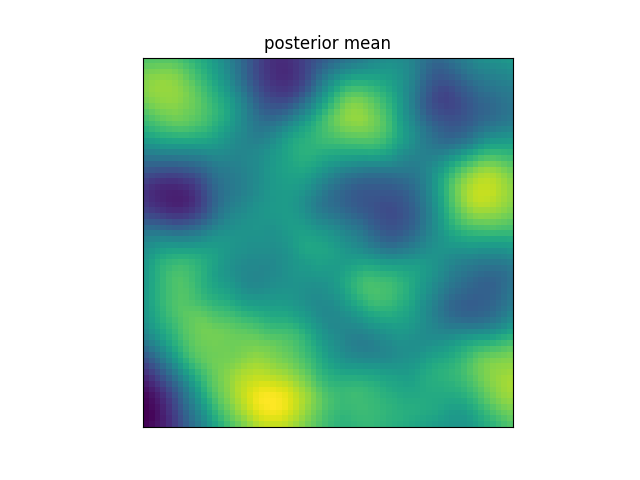
\includegraphics[width=0.72\textwidth]{figures/Figure_14.png}
% \end{center}
% \end{frame}

\begin{frame}{Comparing the Two Synthetic Examples}
Example I has moderate contrast $(4.5,5.5)$, whereas Example II has stronger contrast $(3.5,6.5)$. Both are reconstructed using the same latent Gaussian Poisson model.
\begin{columns}[T]
\begin{column}{0.52\textwidth}
\begin{center}
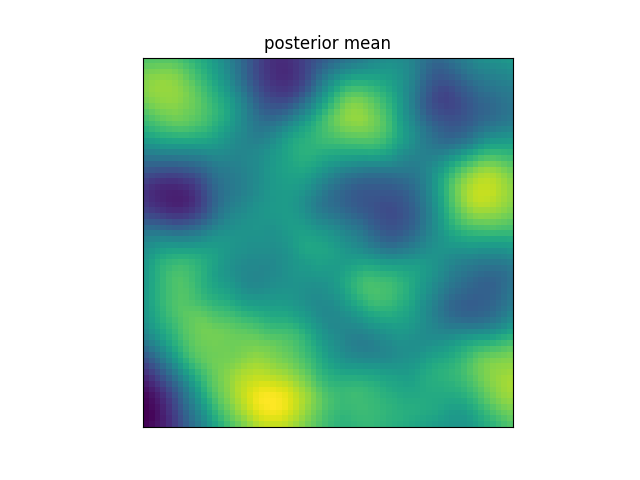
\includegraphics[width=\textwidth]{figures/Figure_14.png}

\scriptsize posterior mean, example I
\end{center}
\end{column}
\begin{column}{0.52\textwidth}
\begin{center}
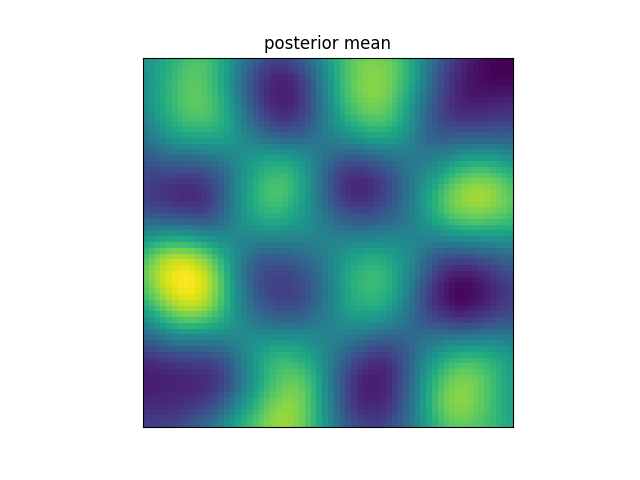
\includegraphics[width=\textwidth]{figures/Figure_7.png}

\scriptsize posterior mean, example II
\end{center}
\end{column}
\end{columns}

\end{frame}

% -------------------------------------------------
\section{Takeaways}

\begin{frame}{Takeaways}
\begin{itemize}
\item Point events can be modeled via latent spatial Poisson fields.
\item A Gaussian prior on $f$ induces flexible rate priors.
\item Poisson splitting converts the model into a logistic form.
\item P\'olya--Gamma augmentation then restores conditional Gaussian structure.
\item Gibbs sampling becomes efficient via Cholesky updates.
% \item The framework extends naturally to real earthquake data and adaptive grids.
\end{itemize}
\end{frame}


\begin{frame}{Outlook}
Future directions:
\begin{itemize}
\item Quadtree / adaptive grids
\item Sparse precision matrices
\item Nonstationary covariance kernels
\item Real earthquake catalogs
\item Spatio-temporal extensions
\end{itemize}
\end{frame}

\begin{frame}{Limitations of the Sigmoid Link}
The sigmoid link is useful because it guarantees positivity and gives a tractable P\'olya--Gamma Gibbs sampler.

\medskip
However, it also introduces limitations:
\begin{itemize}
\item the intensity is bounded by the fixed scale parameter $\lambda$,
\[
0<\lambda_i<\lambda,
\]
\item large positive values of $f_i$ are compressed due to saturation,
\item the P\'olya--Gamma variables change in every iteration, so the Gaussian update requires repeated linear algebra,
\item the upper bound may be restrictive for data sets with strongly varying event rates.
\end{itemize}

\medskip
This motivates considering alternative positive link functions.
\end{frame}

\begin{frame}{Beyond the Sigmoid Link}
A natural next question is:
\[
\text{Can we keep positivity while avoiding the fixed upper bound?}
\]

\medskip
One possible alternative is the softplus / soft-ramp link:
\[
\lambda_i = \log(1+e^{f_i}).
\]

\medskip
It remains positive, but grows approximately linearly for large $f_i$.

\begin{block}{Next part}
Cristina presents an alternative inference strategy based on this softer, unbounded link function.
\end{block}
\end{frame}

\begin{frame}{Thank you}
\begin{center}
\Large Thank you for your attention!\\[1em]
Questions?
\end{center}
\end{frame}

% -------------------------------------------------
\appendix
\section{Appendix}

\begin{frame}{Appendix: Synthetic Example II -- Event Catalog}
\begin{center}
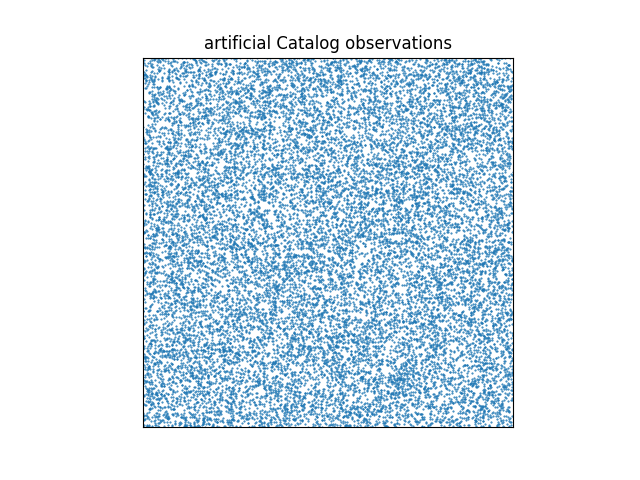
\includegraphics[width=0.72\textwidth]{figures/Figure_10.png}
\end{center}
\end{frame}

\begin{frame}{Appendix: Synthetic Example II -- Gaussian First Guess}
\begin{center}
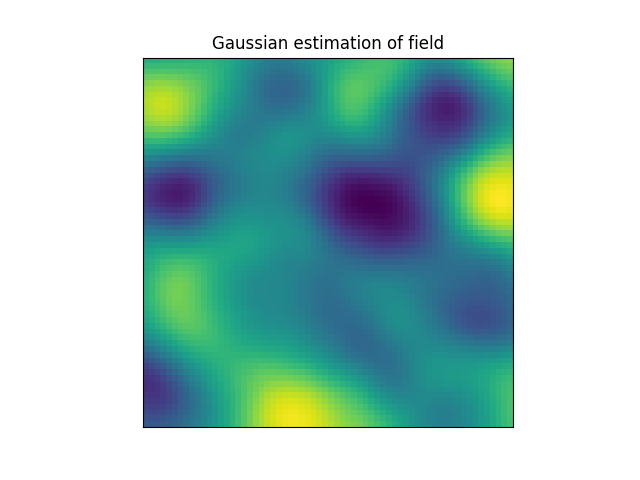
\includegraphics[width=0.72\textwidth]{figures/Figure_12.png}
\end{center}
\end{frame}

\begin{frame}{Appendix: Synthetic Example II -- Posterior Samples}
\begin{center}
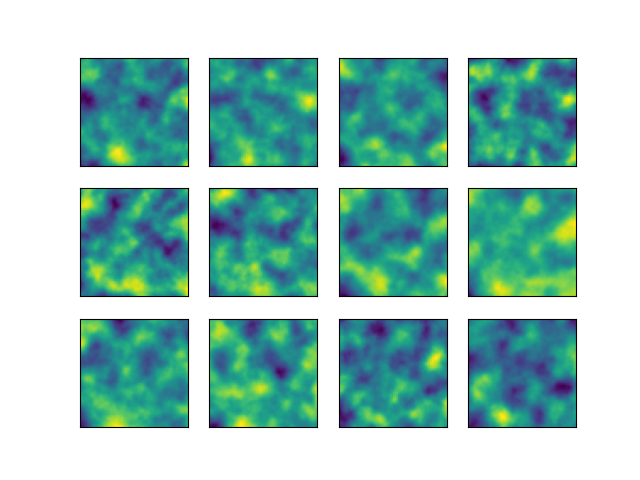
\includegraphics[width=0.82\textwidth]{figures/Figure_13.png}
\end{center}
\end{frame}

\begin{frame}{Appendix: Real Earthquake Data}

Possible discussion points:
\begin{itemize}
\item real point process data
\item spatially varying seismic activity
\item comparison with synthetic experiments
\end{itemize}
\end{frame}

\begin{frame}{Appendix: Adaptive Grid / Quadtree}

Possible discussion points:
\begin{itemize}
\item more cells where the data are dense
\item fewer cells where the data are sparse
\item rates must be interpreted relative to cell area
\end{itemize}
\end{frame}

\end{document}